\documentclass[runningheads,a4paper]{llncs}
\usepackage{amssymb}
\setcounter{tocdepth}{3}
\usepackage{graphicx}
\usepackage{multirow}
\usepackage{booktabs}
\usepackage{algorithm2e}
\usepackage [english]{babel}
\usepackage [autostyle, english = american]{csquotes}
\MakeOuterQuote{"}
\usepackage{float}

\renewcommand\dblfloatpagefraction{.99}
\renewcommand\dbltopfraction{.99}
\renewcommand\floatpagefraction{.99}
\renewcommand\topfraction{.99}
\renewcommand\bottomfraction{.99}
\renewcommand\textfraction{.01}

\usepackage{url, listings, color} 
\newcommand{\keywords}[1]{\par\addvspace\baselineskip
\noindent\keywordname\enspace\ignorespaces#1}

\definecolor{mygray}{rgb}{0.95,0.95,0.95}
\lstset{frame=none,
  backgroundcolor=\color{mygray},
  language=Octave,
  aboveskip=3mm,
  belowskip=3mm,
  showstringspaces=false,
  columns=flexible,
  basicstyle={\small\ttfamily},
  xleftmargin=15pt,
  numbers=left,
  breaklines=true,
  breakatwhitespace=false,
  tabsize=2,
}

\begin{document}

\title{A Comparative Analysis of Eclipse Modelling Git Repositories}
\author{Daniel Brown\and Dimitrios S. Kolovos}
\institute{Department of Computer Science, University of York, United Kingdom \\ \{dtb508,dimitris.kolovos\}@york.ac.uk}
\maketitle

\begin{abstract}
Git is one of the most popular version control systems available \cite{gitpopularity} and, as well as many privately hosted instances, powers the well-known social programming website GitHub \cite{gitpowersgithub}.

Despite Gits popularity there are few systems available for analysing a git repository or querying it for useful metrics such as most popular commit time, largest commit, most active contributor or something more complex.

The systems that do exist to analyse Git repositories, namely GitInspector \cite{gitinspector} and Github, don't allow for custom queries to be written by the user. Meaning, for example, you cannot ask the question "What day of the week is Daniel most likely to author a commit of over 100 lines" or "Which contributor has had the highest percentage of their committed lines changed by someone else". 

This workshop presents a tool, called EpsilonGit, which allow users to write these custom queries by letting them interact with a git object database as a model using the Epsilon platform and its associated domain specific modelling languages. This model-based solution is then used to make some basic queries against some Eclipse Modelling Git repositories.
\end{abstract}

\section{Introduction}
Git is a free and open source distributed version control system \cite{gitintro} that is designed to allow users to manage changes to files, often source files in a software project. This enables developers to "roll back" to a previous version of a file, see the difference between a file at two different times or determine which team member authored a line of code. 

Version control best practices suggest that a developer should be committing code a little at a time and quite often \cite{gitbestpractices}, this makes it a good place to analyse to determine an individual developer or teams working practices in retrospect.

A project manager may want to analyse a git repository to answer questions such as "How large is the average commit size?", "What time of the day are most commits made?" and "Which of my developers is committing the most code that is later replaced?". The answers to these questions may allow improvements in both quality of code and workplace practices.

Mining Software Repositories (MSR) for information to improve Software Engineering practices is a hot area of research right now with an annual dedicated conference \cite{msr2015}. MSR is the process of analysing the rich data available in these repositories to uncover interesting and actionable information about software systems \cite{theroadagainformsr} including identifying pre-existing patterns in code, and automatically linking code to bug reports -- this project aims to aid that discovery. Answering semantically challenging questions such as "Does the git fork flow enable more people to contribute to this project?" could be achieved, potentially changing the shape and attitudes of organisations.

Whilst MSR is a popular research topic a recent paper enumerating the tools used by MSR researchers found that many MSR researchers are using general purpose data mining tools rather than bespoke specialised MSR tools \cite{toolsinminingsoftwarerepositories}.

Model Driven Engineering is an approach to tackle the complexity of data, and how it is interacted with, through the use of high level abstractions called models \cite{modeldrivenengineering} and a set of Domain-specific modelling languages and Transformation engines and generators.   
	
Due to the large array of features provided by git and the widespread use of hashes and graph data structures in the underlying system it is often considered to be complex \cite{gitcomplex}\cite{githard}\cite{gitmixedmetaphors}.

Epsilon is a family of languages and tools for code generation, model-to-model transformation, model validation, comparison, migration and refactoring \cite{epsilonhomepage}. Whilst Epsilon comes with support for interacting with EMF, XML and several other types of model formats out-of-the-box it also has a system called the Epsilon Model Connectivity layer which allows developers to implement drivers for other types of models and structured artefacts.

\begin{lstlisting}[caption=List Authors by Number of Commits in Git Bash, label=lst:gitbash]
git log --format='\%aN <\%aE>' | awk '{arr[\$0]++} END{for (i in arr){print arr[i], i;}}' | sort -rn | cut -d\ -f2-
\end{lstlisting}

The project being introduced, EpsilonGit, is a driver for Epsilon to enable developers to work on git at a high level abstraction provided by modelling languages to make the job of querying and analysing git repositories conceptually easier. Currently most people "query" their git repositories by viewing their git log or, if they're looking for something more in-depth resulting to complex scripting like that seen in Listing \ref{lst:gitbash} -- EpsilonGit aims to make writing queries for git simpler, more concise and easier to understand.

\section{Background}
\subsection{The Git Object Model}
The core of git is a content-addressable filesystem which can store any object and assign it a hashcode by which it can be identified \cite{progit}. There are 4 main types of object stored in this system, known as the git object model, which are shown in Figure \ref{fig:gitobjectmodeldiagram}.

\begin{figure}[h]
	\centering
	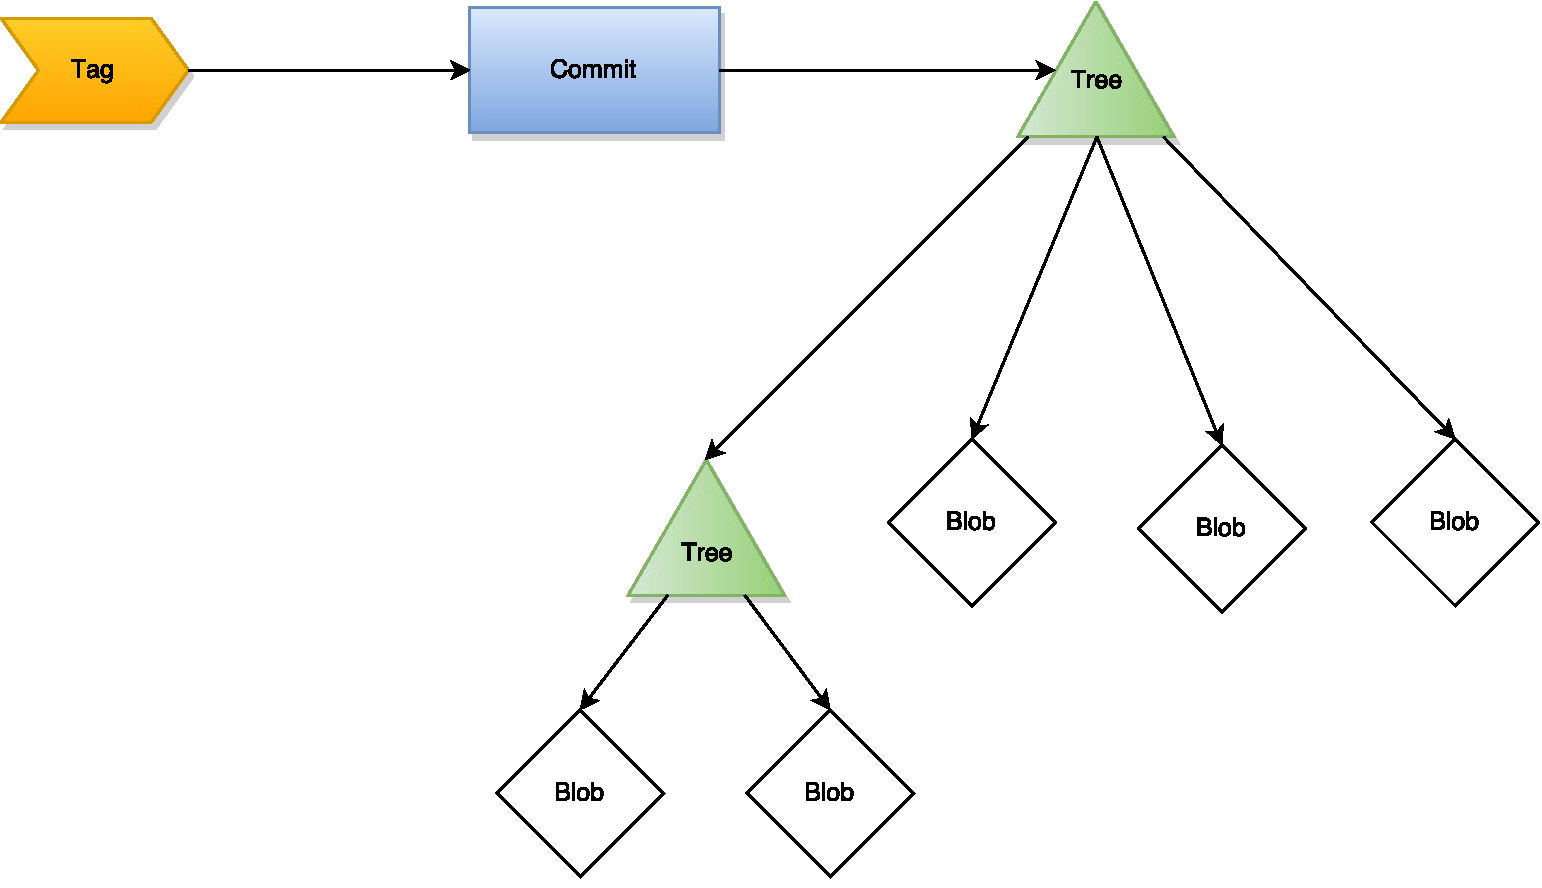
\includegraphics[width=0.7\textwidth]{../thesis/images/gitobjectmodel}
	\caption{The relationships between Git Objects}
	\label{fig:gitobjectmodeldiagram}
\end{figure} 

\subsubsection{Blob}
In git a blob is an array of bytes, which can be text or binary data, that is stored in the content-addressable file system. Blobs should not be confused with files as they are just content with no metadata such as filename, in fact if two files are added to git with exactly the same content, and therefore hashcode, they share a blob.

\subsubsection{Tree}
A tree object in git can be thought of as analogous to a directory in a UNIX file system. For each file in the tree a tuple is stored of the name of file, the hashcode of the blob which contains its content, and a numeric file type code \cite{gitmagic}.

A tree can also contain the names and hashcodes of other trees, allowing for a hierarchical file system, as shown in Figure \ref{fig:gitobjectmodeldiagram}. 

\subsubsection{Commit}
The commit object type stores information about a snapshot of the blobs and trees in the git repository at a particular time. The information includes the name and email address of the author of changes, the name and email address of the person who made the commit, the UNIX timestamp of the time the commit was made, and a message to explain why changes have been made.

A commit points at one-and-only-one root tree, which contains all the other trees and blobs that form part of that snapshot.

\subsubsection{Tag}
Tags specify points in history as being important. Typically people use this functionality to mark release points (v1.0, and so on) \cite{gitdocstags}. They contain the hashcode of the 1-and-only-1 commit they point to, a name (such as "v1.0") and a message explaining why the tagged commit is important \cite{gitforcomputerscientists}.

\subsection{Model Driven Engineering}
Model Driven Engineering (MDE) is an approach to tackle the complexity of data, and how it is interacted with, through the use of high level abstractions called models \cite{modeldrivenengineering} and a set of Domain-specific modelling languages and Transformation engines and generators. "A model is a description of a (part of) systems written in a well-defined language. A well-defined language is a language with well-defined form (syntax), and meaning (semantics), which is suitable for automated interpretation by a computer" \cite{mdaexplained}.

\section{Querying Git Repositories with Epsilon}

\section{Analysis of Eclipse Modelling Git Repositories}
Compute and present statistics related to the size/activity in the Git repositories of the main Eclipse modelling repositories:

\begin{itemize}
  \item git://git.eclipse.org/gitroot/m2t/org.eclipse.jet.git (JET2)
  \item git://git.eclipse.org/gitroot/m2t/org.eclipse.acceleo.git (Acceleo)
  \item https://github.com/eclipse/xtext.git (Xtext)
  \item git://git.eclipse.org/gitroot/epsilon/org.eclipse.epsilon.git (Epsilon)
  \item git://git.eclipse.org/gitroot/mmt/org.eclipse.atl.git (ATL)
  \item https://git.eclipse.org/r/sirius/org.eclipse.sirius (Sirius)
  \item git://git.eclipse.org/gitroot/mmt/org.eclipse.qvto.git (QVTo)
  \item https://git.eclipse.org/r/emf/org.eclipse.emf (EMF)
  \item https://git.eclipse.org/r/incquery/org.eclipse.incquery (IncQuery)
  \item https://git.eclipse.org/r/gmf-tooling/org.eclipse.gmf-tooling (GMF Tooling)
  \item git://git.eclipse.org/gitroot/gmf-runtime/org.eclipse.gmf-runtime.git (GMF Runtime)
  \item git://git.eclipse.org/gitroot/gmf-notation/org.eclipse.gmf.notation.git  (GMF Notation)
  \item https://git.eclipse.org/r/ocl/org.eclipse.ocl (OCL)
  \item https://git.eclipse.org/r/henshin/org.eclipse.emft.henshin (Henshin)
  \item git://git.eclipse.org/gitroot/m2t/org.eclipse.xpand.git (Xpand)
  \item https://git.eclipse.org/r/papyrus/org.eclipse.papyrus (Papyrus)
  \item git://git.eclipse.org/gitroot/uml2/org.eclipse.uml2.git (UML2)
\end{itemize}

\section{Conclusions and Further Work}
Model-Driven Engineering has proven itself to be a highly effective way of dealing with complex structured data -- both in terms of reducing query complexity and enabling more bespoke and complex queries -- and the author thinks that model-driven engineerings role in mining software repositories should be further researched. Performance tests also found that a model driven interface was comparable to and in some cases faster than other git analysis solutions.

Whilst the current design and implementation of EpsilonGit matches the requirements set out for this project it would be possible for a future project to build on the work completed for this one to improve EpsilonGit in a number of ways. 

Currently the system provides read only access to git repositories -- this was all that was required to provide query and analysis tools. If the project was continued it would be possible to add write access via the domain specific languages provided by Epsilon. This could allow the following functionality:

\begin{enumerate}
	\item Authoring of commit messages
	\item Deletion of commits by using the `git reset` command \cite{gitreset}
	\item Managing of merging and branching
	\item Retrospectively changing the name or contact details of authors and committers in the system using git mailmap \cite{gitmailmap}
\end{enumerate} 

It is unknown if there would be benefit to a user in having a model driven interface for making changes to a git repository -- this too could be researched. 

A larger addition to EpsilonGit could be to make it compatible with other popular version control systems -- such as Mercurial and Apache Subversion. Adding in compatibility with these systems, alongside write support, would enable the use of EpsilonGit to migrate from one version control system to another, as well as providing the analysis and querying functionality presented in this report for git.

\bibliographystyle{splncs03}
\bibliography{references}

\end{document}
